\documentclass[12pt]{report}

% Packages
\usepackage[a4paper,width=160mm,top=23mm,bottom=25mm]{geometry} % page layouting
\usepackage[utf8]{inputenc}
\usepackage[english]{babel} % correction
\usepackage{natbib} % 
\usepackage{graphicx} % allows including pictures
\usepackage{titlesec} % custom title page
\usepackage{tabto} % allows using tab
\usepackage{fancyhdr} % to include header
\usepackage{lastpage} % get side number of last page
\usepackage{pgfplots} % table lpot from data
\usepackage{url}
\usepackage{caption}  % multiple images as one
\usepackage{subcaption}
\usepackage[parfill]{parskip} % skip offset on pargraph beginning
\usepackage{float}
\usepackage{glossaries}
\usepackage{outlines}

% syntax highlighting with minted
\usepackage{minted}
\usemintedstyle{vs}
\definecolor{bg}{rgb}{0.95,0.95,0.95}

\newminted{kotlin}{%
    breakbytoken,%
    breaklines,%
    autogobble,%
    label=,%
    xleftmargin={5pt},%
    xrightmargin={10pt},%
    framesep=2\fboxsep,%
    bgcolor=bg,%
}


\graphicspath{ {images/} }

% Bibliography formatting
\bibliographystyle{abbrvnat}
\setcitestyle{authoryear,open={(},close={)},aysep={,}}

% Footer and Header
\pagestyle{fancy}
\fancypagestyle{plain}{}
\fancyhf{}
\rhead{IP6 - Compose Workbench}
\lhead{
\includegraphics[scale=0.9]{fhnw_e_10mm.jpeg}}
\rfoot{\thepage/\pageref{LastPage}}
\fancyheadoffset[L,R]{12mm}

% Formatting
\titleformat{\chapter}{\normalfont\huge}{\thechapter.}{20pt}{\huge\it}

% title hierarchy
% -1	\part{part}
% 0	\chapter{chapter}
% 1	\section{section}
% 2	\subsection{subsection}
% 3	\subsubsection{subsubsection}
% 4	\paragraph{paragraph}
% 5	\subparagraph{subparagraph}

% Document attributes
\newcommand\authorA{Sven Böhm}
\newcommand\authorB{Dominik Frei}
\newcommand\closinglocation{Windisch}
\newcommand\closingdate{12. August 2022}


\begin{document}

\begin{titlepage}   
\vspace*{-18mm}\hspace*{-7mm}
\includegraphics[scale=1.7]{fhnw_e_10mm.jpeg}

    \begin{center}
        \vspace{8mm}
        \Huge
        \textbf{Compose Workbench}
        
        \LARGE
        Bachelor Thesis - IP6
        
        \begin{figure}[H]
            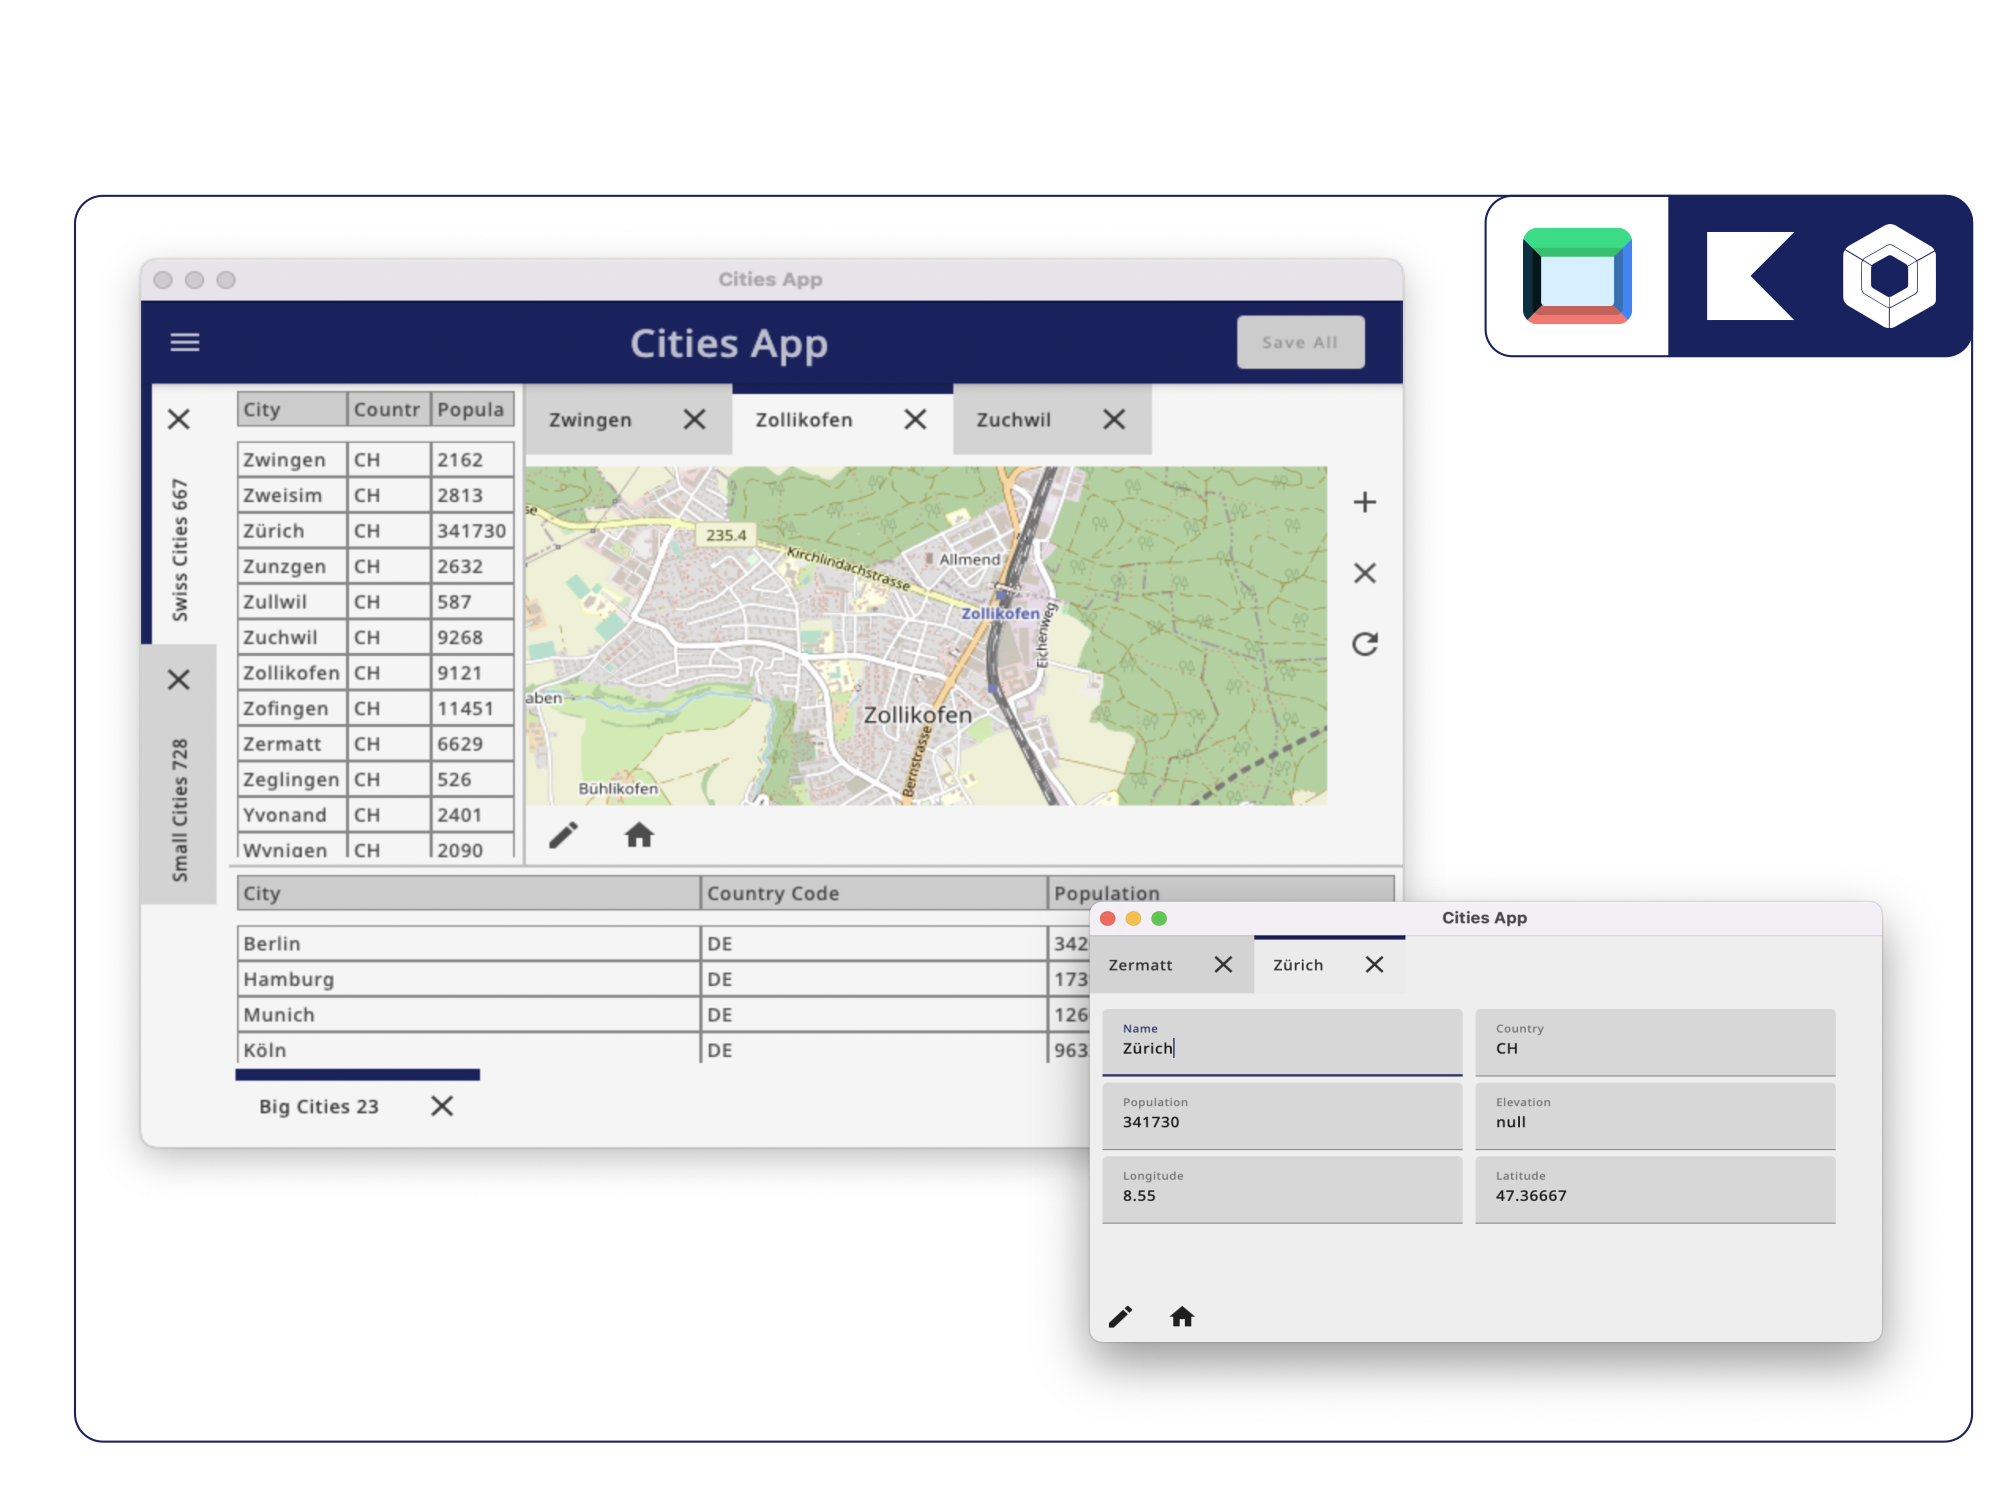
\includegraphics[width=1\linewidth]{images/image-title-3.png}
        \end{figure}

        \vspace{6mm}

        \Large
        \textbf{University of Applied Sciences and Arts Northwestern Switzerland}\\[5pt]
        Computer Science\\[6pt]
        \closinglocation, \closingdate
    \end{center}
    \vspace{6mm}
    \large
    \textbf{Students:} \tab \authorA, \authorB\\[3pt]
    \textbf{Expert:} \tab Dipl.-Inform. Dirk Lemmermann\\[3pt]
    \textbf{Professor:} \tab Dr. Dieter Holz\\[3pt]
\end{titlepage}


\chapter*{Abstract}
In the context of this Bachelor Thesis, a Workbench had to be developed as a library which is designed to integrate user-defined Modules. The Workbench consists of a Workbench-specific Top and MenuBar, which enables global actions (e.g. Save All, Close All), as well as modules that are displayed within one or more tabs. 
In the case of a Module, a conceptual distinction is made between Explorer and Editor. The Explorer is an open context in which mainly data is to be displayed for an overview. The Editor is a typified context that is used to edit data.
The technology of the Workbench is limited to Jetpack Compose Desktop and so only supports Composable Desktop modules. 

The work has an exploratory character. In an initial design and planning phase, an Interaction Guide with wireframes was created to set the approximate workload and features. This formed a solid basis for further development and collaboration. Afterwards, through regular exchange with Professor Dr. Holz, requirements and ideas were continuously added and adapted. 
There was also a strong focus on concepts and architecture for the implementation of features.

With the library developed, user-defined modules can be integrated into the Workbench in a lightweight way and with minimal programming effort. Care was taken to ensure that no exchange of code must or even can take place. All code sources must be able to be used unchanged.
For this purpose, interfaces are implemented by callbacks or the internal MQ messaging system. The MQ messaging system works similar to a REST API and can also be used between independent user-defined modules.

Another achievement is the clean implementation of the MVC architecture with unidirectional data flow. The Model forms an immutable state that contains all the data for the View. This has the advantage that only one object needs to be stateful and the recompose of Jetpack Compose is only managed at one point.
The same applies to the events from the View. These are called as actions via a single method on the controller. This single point of entry into the controller also eased the implementation of concurrent execution of actions on the controller. This means that computationally intensive actions do not block the View.

Compose Workbench provides a library that allows the user to integrate custom modules with little effort. 
Furthermore, the architecture of the workbench is easy to expand, which eases its further development.


\chapter*{Ehrlichkeitserklärung}

Hiermit versichern wir, dass wir diese Projektarbeit selbstständig verfasst und keine anderen als die angegebenen Quellen und Hilfsmittel benutzt haben. Die Stellen unserer Arbeit, die dem Wortlaut oder dem nach Werken entnommen sind, haben wir in jedem Fall unter Angabe der Quelle als Entlehnung kenntlich gemacht. Dasselbe gilt sinngemäss für Tabellen, Abbildungen und Code. Diese Arbeit hat in dieser oder einer ähnlichen Form nicht im Rahmen einer anderen Prüfung vorgelegen.

\vspace{12mm}

\noindent \closinglocation, \closingdate

\vspace{8mm}

\noindent \authorA \hfill \authorB \hfill 

\tableofcontents

\newpage

\chapter{Introduction}
\section{Introduction}
The Compose Workbench is a library which enables the consolidation of existing Modules into one cohesive application. The Compose Workbench provides standard elements like a top bar, tab handling, window management and internal information exchange.

\section{Project Requirements}
The Compose Workbench supports two types of Modules, Explorer and Editor. Explorers are used to display data whereas an Editor is used to edit a specific data record. Explorers should be able to request Editors for specific data records and there should be the possibility to have different Editors for the same type of data.

The Compose Workbench has its own messaging system to send and receive messages from all Modules.

The requirements and especially the usability is more detailed in the chapter \emph{Interaction Guide}.

\section{Technical Requirements}
The Compose Workbench has to be written in Kotlin in combination with JetBrains Compose Desktop.

The embedded version of HiveMQ must be used for the messaging system.

\chapter{Interaction Guide}
\section{User Groups}
\begin{itemize}
\item Compose Workbench configurator: Developer who creates an Application with the help of the Compose Workbench.
\item Compose Workbench user: User of the application created by the Compose Workbench configurator.
\item Compose Workbench contributor: Developer which contributes towards the Compose Workbench.
\end{itemize}


\section{Compose Workbench Elements}
\subsection{Workbench}
The term Workbench is used to describe the complete application which is built by using the Compose Workbench Library.

\subsection{Module}
A Module represents a displayable element inside the workbench. It can be displayed as a Tab or Window and builds the interface to the workbench. Explorer and Editor are the two types of Modules. 

A Module provides following callback which will expose the Modules internal Model.
\begin{itemize}
    \item onClose: will be called when displayed element is closed.
    \item onSave: will be called when global save from Workbench is called.
\end{itemize}

\subsubsection{Explorer}
An Explorer is a type of Module which is used to Explore data. An Explorer can not be requested from outside the library. As best practice all data in an Explorer should be read only.

\subsubsection{Editor}
An Editor is a type of Module which is used to edit data. Editors can be requested by the Compose Workbench configurator from outside the library. This allows editing dynamic data which is displayed in an Explorer. To request an Editor the Controller of the editable Data must be provided.

\section{UI Elements}

\subsection{Main Window}
Main Workbench View refers to the initial Window which is opened when starting the Application. There ca be only one Instance of the Main Window at any time.

\begin{figure}[H]
    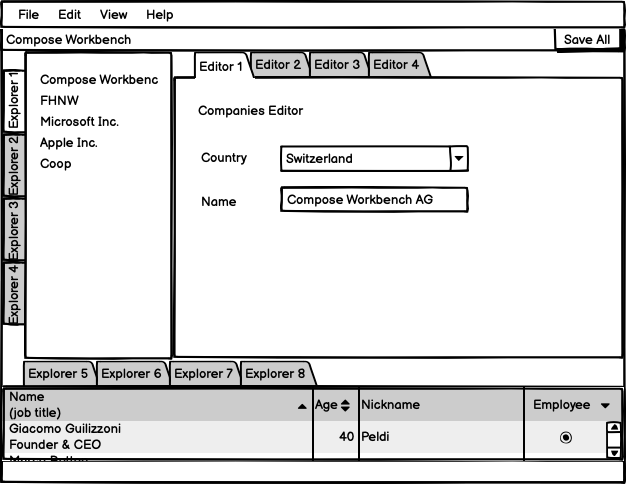
\includegraphics[width=1\linewidth]{images/WorkbenchCompose.png}
    \caption{Overview Main Window}
\end{figure}


The Main Window provides this Actions:
\begin{itemize}
    \item \textbf{Save All}: Sends a save request to all opened Editors.
    \item \textbf{Close}: Closes the Application.
    \item \textbf{Menu Bar}: Workbench specific and Configurator defined Actions are provided.
    \item \textbf{Workbench Menu}: Internal Menu as extension to Menu Bar. Where the Workbench Menu is mention to provide Application specific Actions.
\end{itemize}

\subsection{Tab}
A Tab displays the content of one Module inside the Main Window.

A Tab provides this Actions:
\begin{itemize}
    \item Drag and Drop: Tab can be dragged out of the main Window and dropped into a new Window.
    \item Close: Closes the Tab.
\end{itemize}

\begin{figure}[H]
\centering
\begin{subfigure}{.5\textwidth}
  \centering
  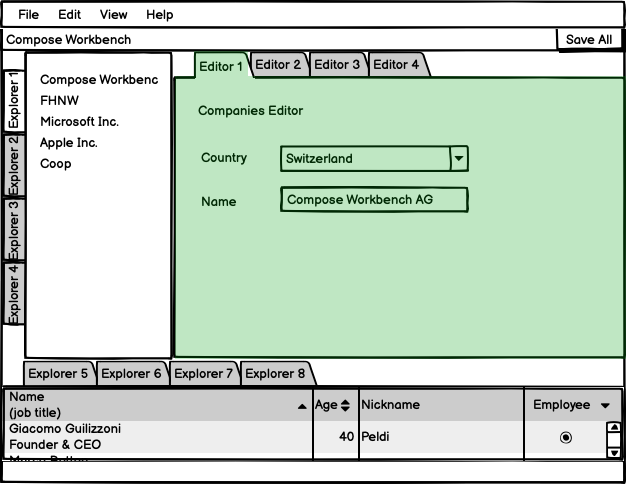
\includegraphics[width=.9\linewidth]{images/WorkbenchCompose (TabToWindow0) (TabToWindow0).png}
  \caption{Drag Tab on TabHeader}
  \label{fig:ransac_result}
\end{subfigure}%
\begin{subfigure}{.5\textwidth}
  \centering
  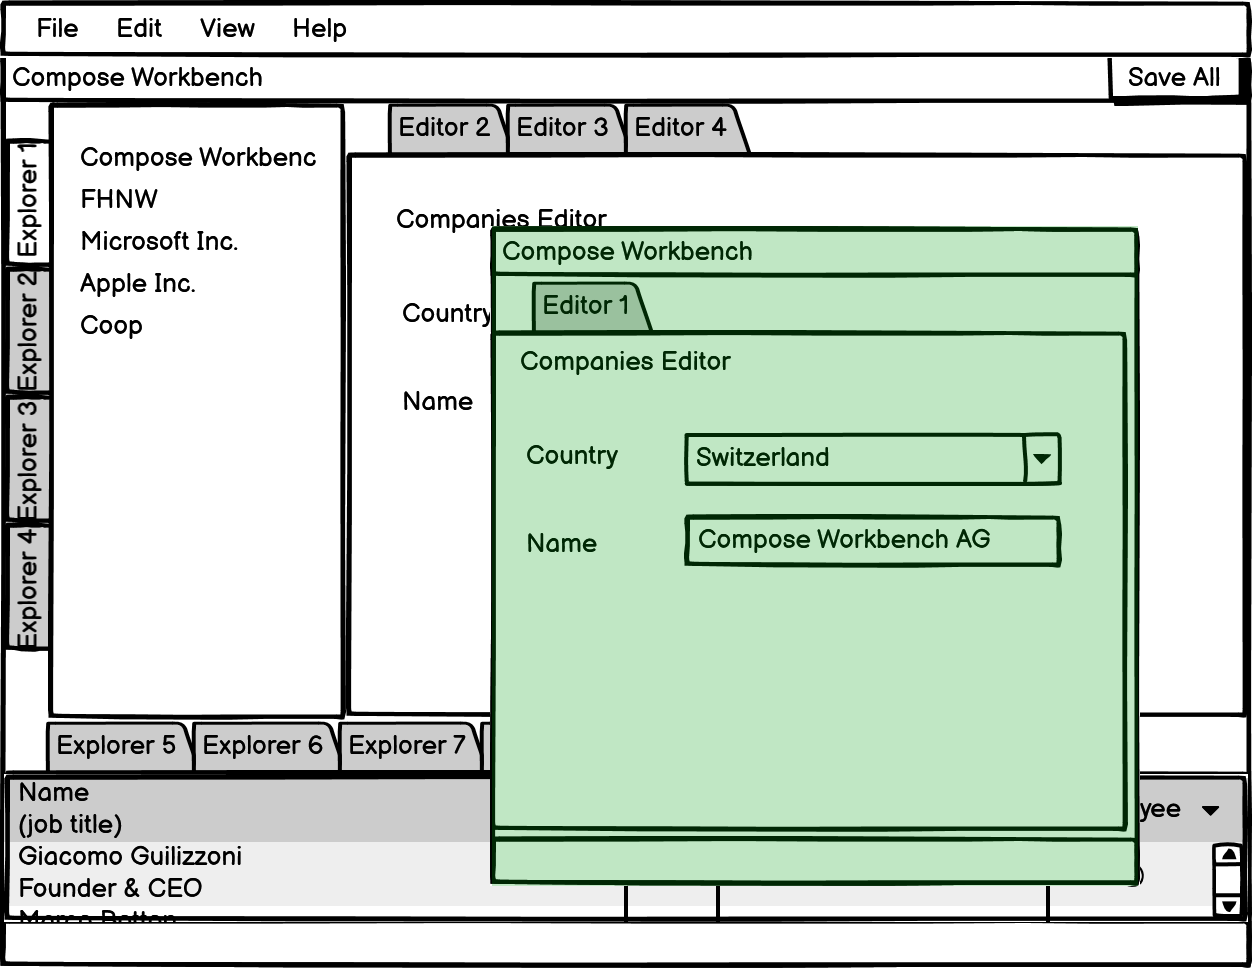
\includegraphics[width=.9\linewidth]{images/WorkbenchCompose (TabToWindow) (TabToWindow).png}
  \caption{Tab is moved out as separate Window}
  \label{fig:ransac_rotation}
\end{subfigure}
\caption{Drag and Drop for Tab/Window}
\label{fig:ransac_results}
\end{figure}

\subsection{Window}
A Window displays the content of one or more Modules outside the Main Window. There can be multiple Windows at the same time, the number of open windows is not limited.


A Window provides this Actions:
\begin{itemize}
    \item Drag: Module from the Window can be dragged back into the main Window or another open Window.
    \item Drop: Module from the main Window can be dropped into the Window
    \item Close: Closes the Window.
\end{itemize}

\subsection{Spaces}
The Workbench Main Window separates two kind of spaces, Editor Space and Explorer Space
\begin{figure}[H]
    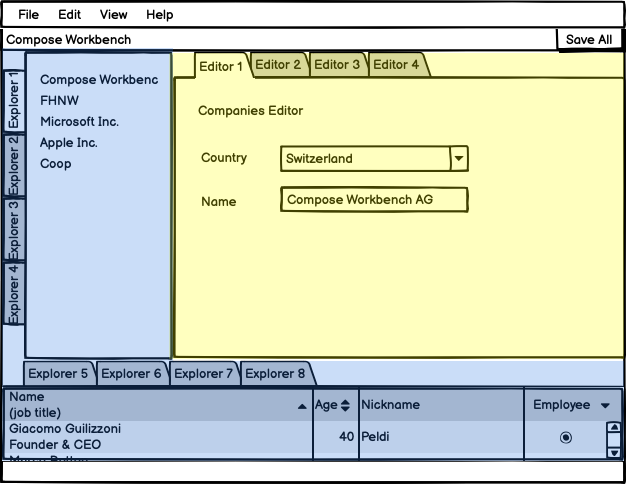
\includegraphics[width=1\linewidth]{images/WorkbenchCompose (SpacesColored) (SpacesColored).png}
    \caption{Editor Space (yellow), Explorer Space, (blue)}
\end{figure}

\subsubsection{Editor Space}


The Editor space displays all opened Editors as Tabs inside of the main Window. The Editor Space can be split once vertically or horizontally to display Editors next to each other. Editors can be moved from one to another split section by Drag and Drop.

\begin{figure}[H]
\centering
\begin{subfigure}{.5\textwidth}
  \centering
  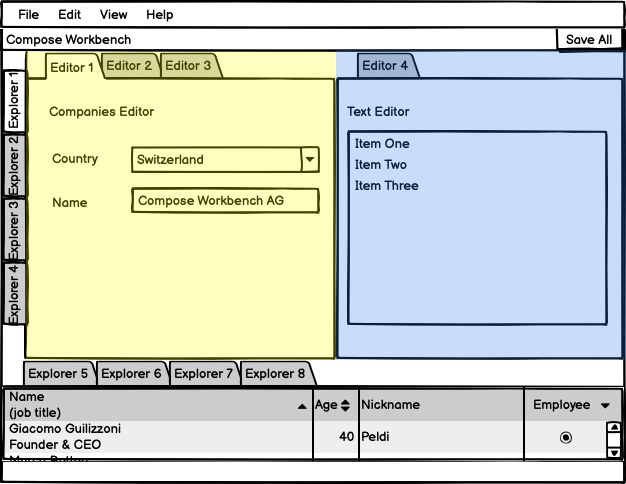
\includegraphics[width=.9\linewidth]{images/WorkbenchCompose (EditorSpaceVerticalSplit) (EditorSpaceVerticalSplit).png}
  \caption{Vertical Split View}
  \label{fig:ransac_result}
\end{subfigure}%
\begin{subfigure}{.5\textwidth}
  \centering
  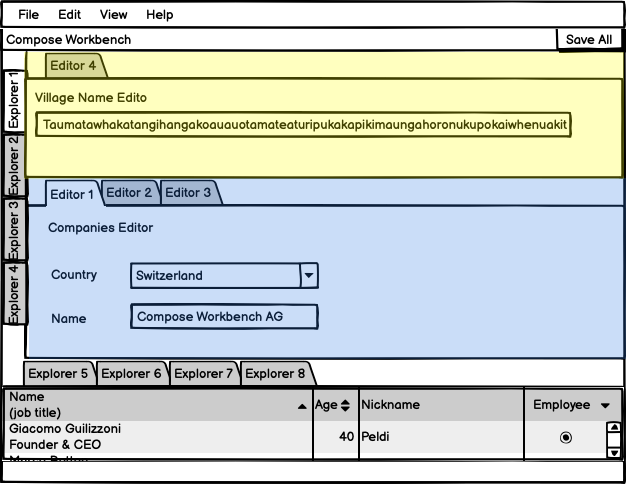
\includegraphics[width=.85\linewidth]{images/WorkbenchCompose (EditorSpaceHorizontalSplit) (EditorSpaceHorizontalSplit).png}
  \caption{Horizontal Split View}
  \label{fig:ransac_rotation}
\end{subfigure}
\caption{Split View on Editor Space}
\label{fig:ransac_results}
\end{figure}


\subsubsection{Explorer Space}

The Explorer space displays all opened Explorers as Tabs. The Explorer Tabs live inside Drawers which can be collapsed. The Explorer space is split into different drawers which have fixed positions (left and bottom). Explorers can be moved from one Drawer to another by Drag and Drop. 

\begin{figure}[H]
\centering
\begin{subfigure}{.5\textwidth}
  \centering
  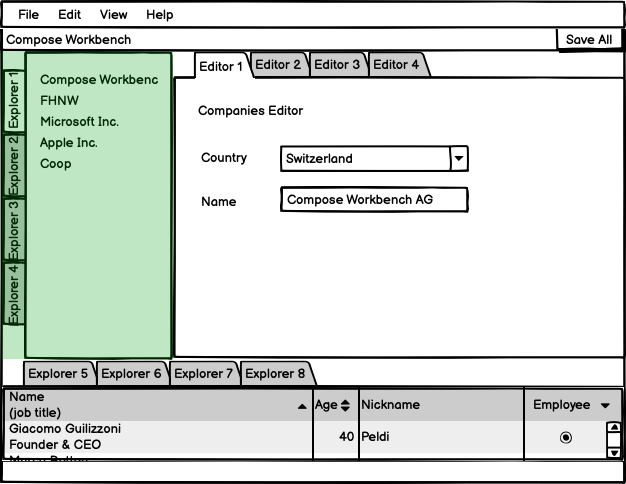
\includegraphics[width=.9\linewidth]{images/WorkbenchCompose (ExplorerSpaceCollapsed0) (ExplorerSpaceCollapsed0).png}
  \caption{Explorer Space open}
  \label{fig:ransac_result}
\end{subfigure}%
\begin{subfigure}{.5\textwidth}
  \centering
  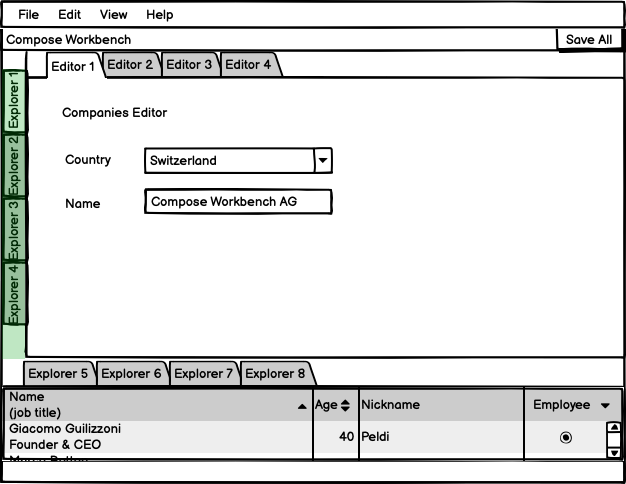
\includegraphics[width=.9\linewidth]{images/WorkbenchCompose (ExplorerSpaceCollapsed) (ExplorerSpaceCollapsed).png}
  \caption{Explorer Space collapsed}
  \label{fig:ransac_rotation}
\end{subfigure}
\caption{Collapsible Explorer Space}
\label{fig:ransac_results}
\end{figure}

\section{Subscribe and Update}
To allow communication between the Workbench Modules, the Workbench supports a topic base subscription and update mechanism. A Module can subscribe to a user defined topic and send updates on user defined topic. The Workbench will come with a set of predefined topics to use.

This mechanism can be used for example to notify about changes done in a editor or to notify about the closing of a editor or explorer.


\chapter{Software Design}
\section{Architecture}
\subsection{Overview}
Jetpack Compose is based on the concept that the View recompose(redraws) itself according to the changes in data state. Therefore the Data/Model we provide to the View has to be wrapped in Mutable States, a Jetpack Compose object which is observed by Compose, which means the View is updated automatically on data change.

With larger applications, a lot of stateful data has to be maintained and updated to keep the View in sync. The data must also be managed and updated correctly to trigger the recompose. For example: changing an item in a list which is wrapped in a Mutable State may not trigger a recompose.

\begin{kotlincode}
var tabs = mutableStateListOf(Tab(1, "Tab1"), Tab(2, "Tab2"))

fun changeTabName1(id: Int, newName: String) {
    tabs.first { it.id == id }?.name = newName
}
\end{kotlincode}

In the example above, you cannot simply change a tab in the list to generate a recompose. Instead, the state only refers to the list. The list must therefore be changed, e.g. by removing the tab to be changed and inserting it again.

\begin{kotlincode}
fun changeTabName(id: Int, newName: String) {
    tabs.removeIf { it.id == id }
    tabs.add(Tab(id, newName))
}
\end{kotlincode}

With an increased number of Mutable States it becomes more complex to maintain an overview of the recomposes triggered with each change. One Recompose can lead to data changes which then in turn trigger other recomposes. The worst case scenario is an infinite recompose loop which impacts the whole application.

To address these problems, we have chosen the approach of the single immutable state. To achieve this an instance of a data class is passed to the view as one state. All members of the class, which are the actual data, are immutable.

\begin{center}
    \begin{figure}[H]
            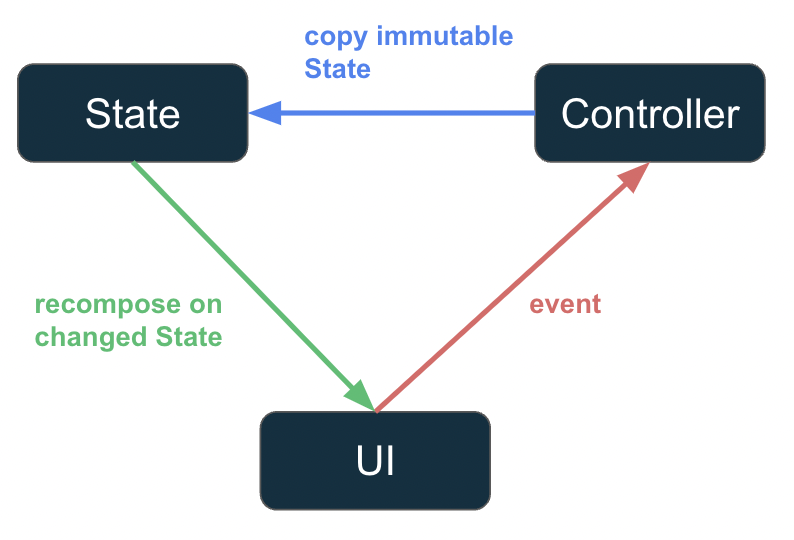
\includegraphics[width=0.6\textwidth]{images/unidirectional data flow.png}
            \centering
            \caption{Unidirectional data flow}
   \end{figure}
\end{center} 

An event from the UI that is to change the data is accepted by the controller. There, a new instance of the data class is created by copying and returned to the view as a new state.
With copy, the members to be changed can be specified as arguments, which allows efficient copying of objects in Kotlin.

This way the recompose is bundled to one point and view, controller and state are cleanly separated. In addition, concurrent changes of state are much easier to handle as they can only be made in one place.


\section{Class Diagram}
\begin{center}
    \begin{figure}[H]
            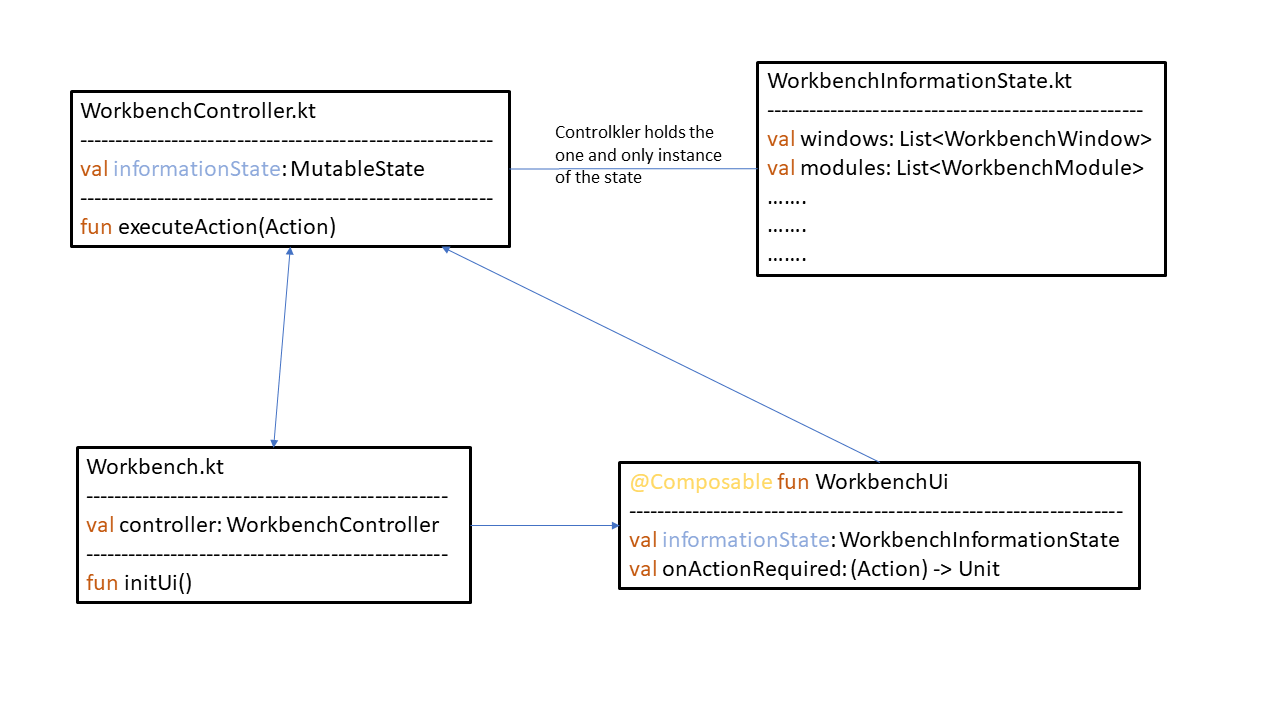
\includegraphics[width=0.8\textwidth]{images/classDiagram.png}
            \centering
            \caption{Simplified classdiagram}
   \end{figure}
\end{center} 

This Simplified class diagram shows the main classes and how they interact.
\begin{itemize}
    \item WorkbenchInformationState: A immutable data class which holds state relevant for the view
    \item WorkbenchController: Holds the only instance of the state as a Mutable State and provides one entry point (executeAction) to manipulate the state
    \item Workbench: The main class which initializes the controller and the view
    \item WorkbenchUi: @Composable function which is the entry point for the Ui
\end{itemize}

The WorkbenchUi receives the state and a callback to execute actions on the controller but not the controller itself to ensure it can only ever call this function. Once executeAction is called the Mutable State in the controller is updated which will trigger a recompose of the WorkbenchUi


\section{Messaging System}
To prevent the exchange of Code from the Workbench and integrated custom Modules or even between custom Modules, but still allow an interaction between those, a Messaging System is provided by the Workbench. 

For the Messaging System an embedded Version of a MQTT Broker is initialized within the Workbench. (https://github.com/hivemq/hivemq-community-edition)
The Address and Port of this Broker are not yet public and cannot be configured by the User. To keep the Messaging System Workbench "internal", a Workbench MqClient is initialized by the Workbench and exposed on certain interfaces, when registering or requesting Workbench Modules.

It is possible to publish (send Messages) and subscribe (receive Messages) to any topic. These actions are called asynchronous and for the subscribe a callback has to be defined to handle receiving messages.

\subsubsection{Topics}

Topics in MQTT are Strings, which are compared to each other to decide if a Client did subscribe for it. To organize Topics MQTT uses / as Sperator, and also offers also Wildcards.
\begin{figure}[H]
\centering
\begin{subfigure}{.5\textwidth}
  \centering
  
\includegraphics[width=.9\linewidth]{images/topic_wildcard_plus.png}
\end{subfigure}%
\begin{subfigure}{.5\textwidth}
  \centering
  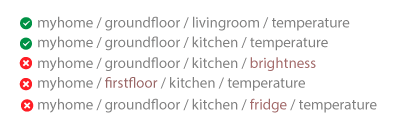
\includegraphics[width=.9\linewidth]{images/topic_wildcard_plus_example.png}
\end{subfigure}
\caption{Wildcard + to access a single level \citep{HiveMQ:MQTT-Essentials}}
\end{figure}

\begin{figure}[H]
\centering
\begin{subfigure}{.5\textwidth}
  \centering
  
\includegraphics[width=.9\linewidth]{images/topic_wildcard_hash.png}
\end{subfigure}%
\begin{subfigure}{.5\textwidth}
  \centering
  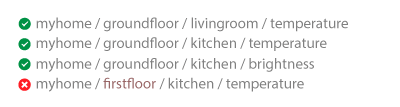
\includegraphics[width=.9\linewidth]{images/topic_wildcard_hash_example.png}
\end{subfigure}
\caption{Wildcard \# to access multi level \citep{HiveMQ:MQTT-Essentials}}
\end{figure}

So it's best practice to use the topics like a REST API, to take full advantage of these features.

For example if you want to publish a change of a Data field of the type City in our CityApp.
\begin{kotlincode}
mqClient.publish("city-app/city/$id/$field", value)
\end{kotlincode}

and on the other side to subscribe to any changes on a City.
\begin{kotlincode}
mqClient.subscribe("city-app/city/#", ::updateTempChanges)
\end{kotlincode}


\section{Asynchronous actions execution}
To prevent blocking the main thread where the UI is running, on executing resource and time consuming actions, it's important to run actions asynchronous. To handle actions asynchronous they have to be queued and must keep their order of execution. For this kind of use Kotlin offers channels. 
On a channel, information (Objects) can be shared between coroutines, by send to and receive from a channel.

A channel provides multiple options for how information is queued and processed. In our case we're using a unlimited buffered channel. Unlimited means that the send is never suspended until the application would run out of memory.
We assume this will not happen, because a Workbench has only few actions being called and most of them can be executed fast.

\begin{center}
    \begin{figure}[H]
            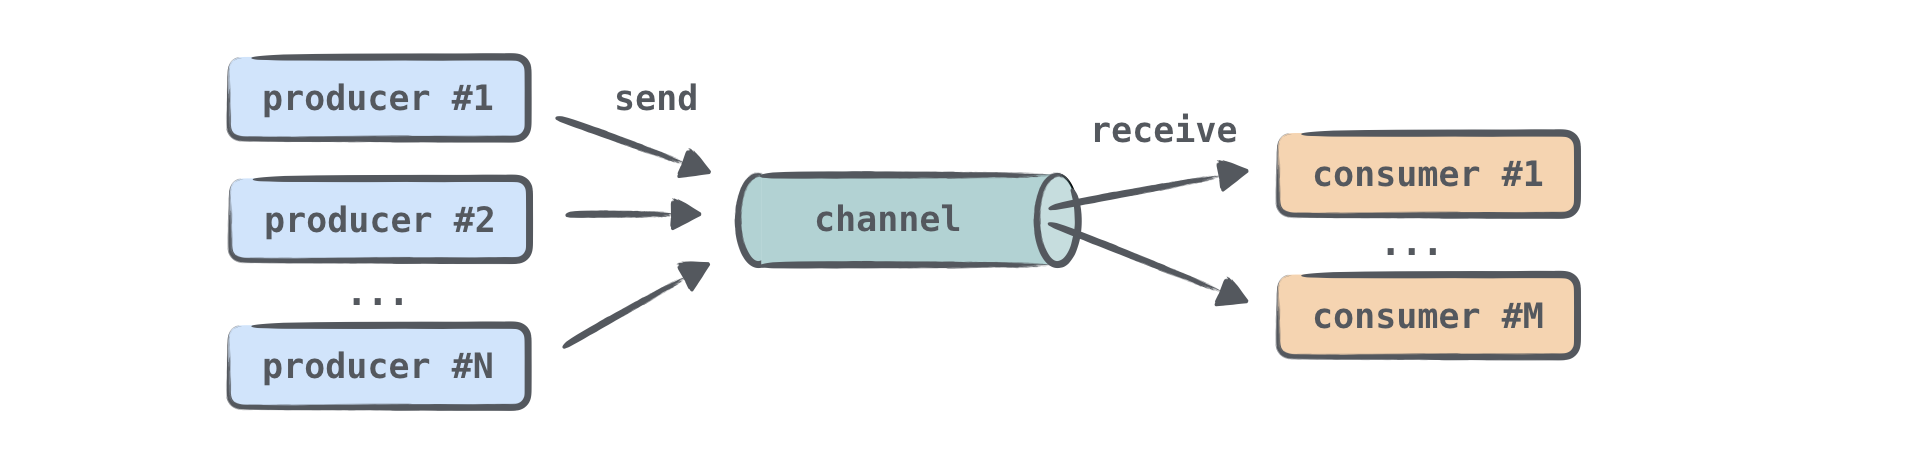
\includegraphics[width=0.7\textwidth]{images/UsingChannelManyCoroutines.png}
            \centering
            \caption{Channel concept in Kotlin \citep{KotlinLang:Playground}}
   \end{figure}
\end{center} 

To guarantee a deterministic behavior of the Controller and its state only one coroutine is receiving actions from the channel and make changes of the state. There would be actors to ensure only one coroutine is receiving message of the channel. But Actor of coroutines are  obsolete, so we skipped using it. 
On the other side any amount of coroutines are allowed to send actions to the channel.

\subsection{Synchronous actions}
Some of the actions have to be executed synchronous, otherwise the correct behavior of the Workbench is not guaranteed. For example a registration of a Module must be synchronous. Otherwise if a request is called before the registration is completed we can't request these kind Modules. 

For the synchronous action a class is introduced which hold a CompletableDeferred as response.

\begin{kotlincode}
internal sealed class WorkbenchActionSync(
    name: String,
    val response: CompletableDeferred<Int> = CompletableDeferred()
): WorkbenchAction(name) 
\end{kotlincode}

The action trigger is waiting for the response to be completed. Because the triggerAction is runBlocking it's caller is blocked until the response is set completed by the actionChannel consumer.

\begin{kotlincode}
private fun triggerAction(action: Action) = runBlocking {
    launch {
        actionChannel.send(action)
    }
    if (action is WorkbenchActionSync) {
        action.response.await()
    }
}
\end{kotlincode}


\section{Trailing lambdas} \label{Traling_lambdas}

According to Kotlin convention, if the last parameter of a function is a function, then a lambda expression passed as the corresponding argument can be placed outside the parentheses \citep{KotlinLang:TrailingLambdas}

This language feature is heavily used throughout Jetpack Compose. For example in UI elements such as columns and rows where the last argument of the Column() function is the actual content of the Column. This allows function calls which look and feel more like functions itself

\begin{kotlincode}
Column {
    Card ( onClick = { println("clicked")}) {
        Text(text = "click me")
    }
}
\end{kotlincode}

In this example, the Card with its text and onClick action is an Argument to the Column function.

In order to make the Workbench consistent with Jetpack Compose and to ensure a easy to use handling the Workbench is also making heavy use of trailing Lambda functions. Trailing Lambdas are used so the user can define the Content of the Modules when registering them. Interaction with the Workbench is done solely using functions.

\chapter{Possible Future Enhancements}
Following are some workbench functionalities which have as of now no solution and do not work. They are however interesting and valuable for the user experience and therefore outlined here as ideas with very high level solutions.

\section{Savable Workbench state}
The Workbench model and with it the complete Workbench state is not accessible by the Workbench configurator. Information such as the currently opened Editors and visible Explorers are not public and cannot be saved.

\subsubsection{Possible Solution}
Introduce a Persistence Data Model (a subset of the Workbench Model) which contains all states worth saving. Add this to the Workbench parameters so existing state can be passed when starting the Workbench and add an on close callback in the Workbench to store the Persistence Data.
\begin{kotlincode}
    val workbench: Workbench = Workbench("App Title", existingData) {
        updatedData ->
            save(updatedData)
    }
\end{kotlincode}
The advantage of this solution is, that access to the Persistence Data can be restricted to the callback function and the actual Workbench Model stays hidden.

\section{Editor for multiple Items}
The interface for requesting Editors restricts the Editor to receive one Item id at a time. For some Editors (e.g. comparison between items) this will not be enough. 
An Editor with multiple Items is not much different to an Explorer. This could become confusing for the users and has to be considered when adding this feature.

\subsubsection{Possible Solution}
The Editor interface accepts a list of ids. This requires some extra checks to make sure the passed id list does at least contain one id at all times.

\section{Aspects}
A third Module Type which is not bound to a data type. This Module handles general Aspects of the Software and is accessible for each Editor. This could be functionality like accessing other resources for a given data record or tracking of external updates.

\subsubsection{Possible Solution}
A possible way to do this is to use the subscribe and update functionality. An Aspect could listen to Editor changes and therefore know once an Editor is opened or selected. Aspects could also define special messages which Editors have to send to provide additional information.

\section{Material Design 3}
Currently the Material Design 2 is used for the Workbench to provide Styling throughout the application. For Jetpack Compose on Android there is Material Design 3 available, which allows more granularity and dynamic Styling. Until now the necessary Libraries are not ported to androidx and is not available for Jetpack Compose cross platform.
As soon JetBrains provides these libraries Material Design 3 will be an interesting option to style the Workbench.

\section{Style Exchange}
To achieve a uniform styling of the Workbench and user-defined modules, the same styling must be exchanged and applied.

\subsubsection{Possible Solution}
The Workbench and user-defined modules have to use the same Material Design. The Material Design has to be defined on Workbench Side and be passed to it's registered modules, so the styling can be applied.


\section{Messaging in between Workbench Clients}
The Messaging System of a Workbench could be used to exchange changes in between Workbench Clients. For example to exchange an unsaved change on the same data field.

\subsubsection{Possible Solution}
There has to be an additional MQTT Broker on a Server to exchange messages in between Workbench Clients. The specific configuration to access the external server and convenience functionality on Workbench side has to be implemented on top of the current messaging system.


\section{Context switch to write State}
The reassignment of State in controller.executeAction must be done in the Main Cortoutine Context, to guarantee thread safety.
Currently the state is reassigned in the Default context, which is using thread pool with other threads then the main thread. 
\begin{kotlincode}
private fun startConsumingActions() {
    CoroutineScope(Dispatchers.Default).launch {
        actionChannel.consumeEach { action ->
            controller.executeAction(action)
            if (action is WorkbenchActionSync) {
                action.response.complete(0)
            }
        }
    }
}
\end{kotlincode}
This carries the risk that the state can be reassigned during a recompose.
Currently, this is prevented because only because the Recompose is finished until the next action is 0one coroutine overwrites the state, so no race conidition is created and the recompose is only triggered if the state is reassigned by this coroutine. 

In order to be thread safe for extensions, this adjustment should be made.

\subsubsection{Possible Solution}

A possible solution would be that the state is no longer a member of the controller but is passed as an argument of an executing action. This execution in turn returns a state and overwrites the previous state in the main context.

\begin{kotlincode}

val state by mutableStateOf(WorbenchState())

private fun startConsumingActions() {
    CoroutineScope(Dispatchers.Default).launch {
        actionChannel.consumeEach { action ->
            val newState = controller.executeAction(state, action)

            witchContext(Dispatchers.Main) {
                state = newState
            }
            
            if (action is WorkbenchActionSync) {
                action.response.complete(0)
            }
        }
    }
}
\end{kotlincode}

We didn't changed the behavior of executeAction, due to the many changes of the controller and it's Unit Test.

\chapter{Alternative Designs}
\section{Workbench integration}
There are other ways in which the workbench integration could be done. The java approach \ref{Use_Of_class_extention} and another Kotlin feature \ref{Use_of_scope_slots}. Both approaches would work and they both have their own advantages and disadvantages.

\subsection{Use of Scope Slots Function} \label{Use_of_scope_slots}
Kotlin supports scoped functions. These functions provide access to the Object and define scopes which can be accessed by the caller.

Instead of having a Workbench object which the user has to create and then use, the Workbench could be a scoped function with scopes for adding Explorers and Editors.

\begin{kotlincode}
createComposeWorkbench() {
    editors{
        editor{
            //define content of editor here
        }
    }
    explorers{
        explorer{
            //define content of explorer here
        }
    }
}
\end{kotlincode}

\subsection{Use of class extension} \label{Use_Of_class_extention}
In contrast to the used trailing lambda approach or the above mentioned scoped functions the workbench integration could be done with a more classical approach of extending and overriding a given class. 

\begin{kotlincode}
class MyWorkbenchEditor(): ComposeWorkbenchEditor {
    
    @Composable
    override fun content(){
        //The actual editor content
    }
}
\end{kotlincode}


\section{Internal Messaging System}
Instead of the embedded HiveMQ Broker and it's Clients, another internal concept could be used. Until now we didn't notice a lack of performance due to the messaging through the embedded Broker (Server). But it can be see as an over kill for a desktop application and may be become critical on larger applications with way more messages.

A internal Messaging System with out a network would be ways faster on transmission and initialization of it's infrastructure.

For example Kotlin's Channels could be an interesting approach to use as a messaging system. Channels offer by default concurrent access by Coroutines and filter for incoming messages. Implementations like BroadcastChannels indicate to use it as network like information exchange.

\chapter{Testing}
Testing is limited to Unit and Usability Tests. It was agreed at the beginning of the project to not do UI testing since this is not so straight forward with Jetpack Compose. 

The Unit test focus on the Controller and the Actions which can be triggered by the View. The test coverage shows no test in the view package but a coverage of 45 of 48 functions in the Workbench Controller Class, which is where most of the logic is.

\begin{figure}[H]
\centering
\begin{subfigure}{.5\textwidth}
  \centering
  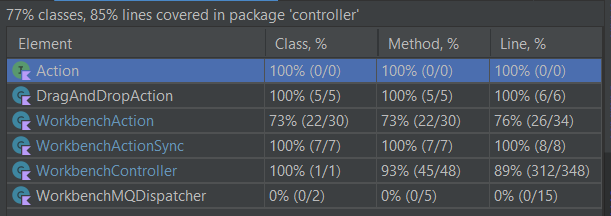
\includegraphics[width=.9\linewidth]{images/TestCoverageControllerPackage}
  \caption{Controller test Coverage}
  \label{fig:ransac_result}
\end{subfigure}%
\begin{subfigure}{.5\textwidth}
  \centering
  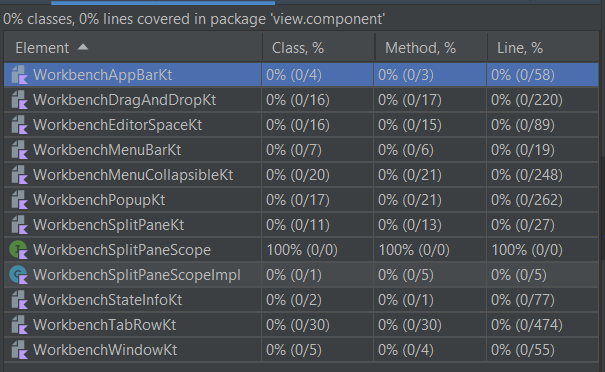
\includegraphics[width=.9\linewidth]{images/TestCoverageViewPackage.PNG}
  \caption{Explorer Space collapsed}
  \label{fig:ransac_rotation}
\end{subfigure}
\caption{View test Coverage}
\label{fig:ransac_results}
\end{figure}

\section{Usability Test}
The real estate example was created by Prof. Dr. Holz as part of a Usability test. This test led to changes around the Modules data handling and initialization.

\chapter{Conclusion}
Starting the project by focusing on the Interaction Guide helped a lot in the development process that came later. It gave a very clear definition of the Modules (Explorers and Editors) and their interactions which was used throughout the project. It also helped in working out the main features and what exactly makes them valuable.

The implementation started with a very limited version of the Compose Workbench which was then enhanced and used as a base for further changes. This approach turned out to be problematic later in the project because it focused on what should be done but not on how it should be done and it left out all the Jetpack Compose specific recompose considerations.

The initial Workspace had a Mutable State for Modules, later came a Mutable State for Windows then one for Commands, PopUps and so on. This lead to problem with the recompose behaviour and was then solved with a global immutable state. This Refactoring took a time and was still compromised by the existing functionality some classes which are part of the state are still mutable as a result of this.

This process led to a couple of findings, which should be considered on any Jetpack Compose project.

\textbf{No mutable objects as part of the state:} This has two benefits, changes to the state cannot happen "by accident" and the recompose is guaranteed with each change.

\textbf{Single point for state mutations:} Restricting access to the state helps in managing all the changes and also in understanding the recompose behaviour. 

\textbf{Group state by recompose effects:} Create different state objects based on the desired recompose behaviour. 



\appendix
\printglossaries

\chapter{Source Code}
\section{Git Repository}

https://github.com/FHNW-IP5-IP6/ComposeWorkbench.git

\bibliography{references}
\end{document}
